%%%%%%%%%%%%%%%%%%%%%%%%%%%%%%%%%%%%%%%%%
% Short Sectioned Assignment LaTeX Template Version 1.0 (5/5/12)
% This template has been downloaded from: http://www.LaTeXTemplates.com
% Original author:  Frits Wenneker (http://www.howtotex.com)
% License: CC BY-NC-SA 3.0 (http://creativecommons.org/licenses/by-nc-sa/3.0/)
%%%%%%%%%%%%%%%%%%%%%%%%%%%%%%%%%%%%%%%%%

%----------------------------------------------------------------------------------------
%	PACKAGES AND OTHER DOCUMENT CONFIGURATIONS
%----------------------------------------------------------------------------------------

\documentclass[paper=a4, fontsize=11pt]{scrartcl} % A4 paper and 11pt font size

% ---- Entrada y salida de texto -----

\usepackage[T1]{fontenc} % Use 8-bit encoding that has 256 glyphs
\usepackage[utf8]{inputenc}
%\usepackage{fourier} % Use the Adobe Utopia font for the document - comment this line to return to the LaTeX default

% ---- Idioma --------

\usepackage[spanish, es-tabla]{babel} % Selecciona el español para palabras introducidas automáticamente, p.ej. "septiembre" en la fecha y especifica que se use la palabra Tabla en vez de Cuadro

% ---- Otros paquetes ----

\usepackage{url} % ,href} %para incluir URLs e hipervínculos dentro del texto (aunque hay que instalar href)
\usepackage{amsmath,amsfonts,amsthm} % Math packages
%\usepackage{graphics,graphicx, floatrow} %para incluir imágenes y notas en las imágenes
\usepackage{graphics,graphicx, float} %para incluir imágenes y colocarlas

% Para hacer tablas comlejas
%\usepackage{multirow}
%\usepackage{threeparttable}

%\usepackage{sectsty} % Allows customizing section commands
%\allsectionsfont{\centering \normalfont\scshape} % Make all sections centered, the default font and small caps

\usepackage{fancyhdr} % Custom headers and footers
\pagestyle{fancyplain} % Makes all pages in the document conform to the custom headers and footers
\fancyhead{} % No page header - if you want one, create it in the same way as the footers below
\fancyfoot[L]{} % Empty left footer
\fancyfoot[C]{} % Empty center footer
\fancyfoot[R]{\thepage} % Page numbering for right footer
\renewcommand{\headrulewidth}{0pt} % Remove header underlines
\renewcommand{\footrulewidth}{0pt} % Remove footer underlines
\setlength{\headheight}{13.6pt} % Customize the height of the header

\numberwithin{equation}{section} % Number equations within sections (i.e. 1.1, 1.2, 2.1, 2.2 instead of 1, 2, 3, 4)
\numberwithin{figure}{section} % Number figures within sections (i.e. 1.1, 1.2, 2.1, 2.2 instead of 1, 2, 3, 4)
\numberwithin{table}{section} % Number tables within sections (i.e. 1.1, 1.2, 2.1, 2.2 instead of 1, 2, 3, 4)

\setlength\parindent{0pt} % Removes all indentation from paragraphs - comment this line for an assignment with lots of text

\newcommand{\horrule}[1]{\rule{\linewidth}{#1}} % Create horizontal rule command with 1 argument of height



\begin{document}
	
	\begin{titlepage}
		\centering
		
\includegraphics[width=0.8\textwidth]{decsai.jpeg}\par\vspace{1cm}
		{\scshape\LARGE Universidad de Granada \par}
		\vspace{1cm}
		{\scshape\Large Recuperaci\'on de Informaci\'on \par}
		\vspace{1.5cm}
		{\huge\bfseries Pr\'actica 1: B\'usqueda de informaci\'on en la web\par}
		\vspace{0.2cm}
		\noindent\rule{\textwidth}{2pt}
		\vspace{2cm}
		{\Large\itshape Miguel \'Angel Torres L\'opez y Luis Balderas Ruiz\par}
		
		\vfill
		
		% Bottom of the page
		{\large \today\par}
	\end{titlepage}
	
	\tableofcontents
	
	\newpage
	
	
	\begin{section}{Formatos de codificaci\'on}
		\begin{subsection}{Codificación de caracteres.}
			La codificación de caracteres es un método indispensable en la informática moderna, ya que nos permite comunicar y almacenar caracteres desde la representación binaria. No obstante, las técnicas de codificación de caracteres son algo más antigua, un ejemplo de ello es el código Morse. \\
			
			Desde el punto vista técnico, entendemos por una codificación de caracteres un sistema por el cual representamos caracteres identificándolos uno a uno con otros símbolos normados. 
		\end{subsection}
		
		\begin{subsection}{Formatos de codificación en informática.}
			En informática, uno de los primeros formatos de codificación que aparece es el ASCII. Este sistema de codificación usa un código de 7 bits, aunque los sistemas actuales están obligados a tomar 8 bits como unidad mínima de almacenamiento. Cada combinación representa un caracter, es decir, tiene 128 caracteres codificados. Este número era suficiente para representar textos en inglés y números, pero pronto quedó expuesta la necesidad de incluir otros caracteres, por ejemplo las caracteres latinos con tildes y otros signos de acentuación. \\
			
			Para ampliar la gama de caracteres y al mismo tiempo mantener la retrocompatibilidad UNICODE\cite{unicode}, el consorcio para la estandarización de codificación de caracteres, creo el formato UTF-8. Este formato es compatible con ASCII, pero difiere en el tamaño que ocupa un caracter. En UTF-8 los caracteres pueden ocupar 1, 2, 3 o 4 segmentos de 8 bits, siendo el primer segmento el mismo que el de ASCII.  Esta nueva codificiación permite representar hasta 1,112,064 caracteres, incluyendo alfabetos occidentales, orientales, símbolos matemáticos e incluso algunos de tipo privado.
			
			En cuanto a rapidez, el formato ASCII está por encima del UTF-8. Aunque a priori vemos que los caracteres tradicionales ocupan igual en los dos formatos, 1 segmento de 8 bits, hay ocasiones en que las posibilidades que nos da UTF-8 entorpezcan la lectura. Por ejemplo, supongamos que tenemos un string 'ABC'. En sendos formatos el string ocuparía 24 bits. Pero acceder al tercer elemento es más costoso en UTF-8, pues tenemos un tiempo adicional al tener que comprobar de que tamaño son los dos primeros caracteres.  \\
			
			Otra codificiación de UNICODE es el UTF-16. Este formato usa 1 o 2 segmentos de 16 bits por caracter, por tanto ya no es compatible con ASCII. No obstante, para lenguajes orientales, como el japonés, la mayoría de los caracteres pueden representarse con 16 bits, lo que aumenta la rapidez de lectura. \\ 
			
			Existe tambien el formato UTF-32, con la obligatoriedad de usar 1 segmento de 32 bits por caracter. Al igual que el anterior, no es compatible con ASCII y además es bastante más pesado e ineficiente, pues muchos bits son desaprovechados. Esto lo convierte en un formato poco usado en la actualidad. \\
			
			Por tanto, los dos formatos más comunes en la actualidad son UTF-8 y ASCII, aunque poco a poco se está incorporando el formato UTF-16 por compatibilidad con los ordenadores de origen asiático.
			
			
		\end{subsection}
		
		\begin{subsection}{Sistemas operativos y sus formatos}
			En esta sección haremos un repaso de los principales sistemas operativos y los formatos de codificiación bajo los que trabajan:
			
			\begin{itemize}
				\item \textbf{Windows}. Fue uno de los primeros sistemas en actualizar el formato de codificación. Actualmente utiliza UTF-16, pero sigue sin funcionar de forma óptima con UTF-8.
				
				\item \textbf{Linux}. Funciona en su mayor parte con UTF-8, aunque dispone de herramientas para cambiar el formato de un archivo. Una de ellas es el comando de termina iconv, que convierte una entrada con un formato a una salida con otro distinto.   
				
				\item \textbf{Mac}. Al igual que Linux trabaja con UTF-8.
				
			\end{itemize}
		\end{subsection}
		
		\begin{subsection}{Temporizaci\'on de b\'usqueda.}
			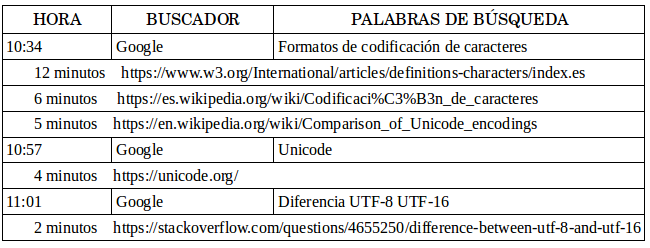
\includegraphics[width=1\textwidth]{codificacion_tiempos.png}
		\end{subsection}
		
	\end{section}


	\newpage
	
	\begin{section}{SEO.}
		SEO (Search Engine Optimization) o posicionamiento en buscadores es uno de los conceptos claves de la industria digital. Tanto el posicionamiento en sí como la profesión que subyace, el SEO se ha convertido en algo que todo empresario, experto en marketing o incluso \textit{influencer} desea entender, manejar o, en el peor de los casos, contratar. En este pequeño informe tratamos de clarificar qué es exactamente el posicionamiento en buscadores desde un punto de vista técnico y por qué es necesario para los afamados \textit{e-business}, así como cuál es el camino para convertirse en un profesional SEO.
		
		\subsection{SEO como herramienta de marketing digital}
		Tal y como \cite{redevolution} menciona, SEO es ``el nombre que se le da a la actividad que intenta mejorar los rankings en las búsquedas", es decir, la posición en la que una página web aparece tras realizar una búsqueda con palabras clave (keywords) relacionadas con dicha web. Hay que añadir que, pese a que nuestra web tenga un gran posicionamiento en buscadores, fruto de un trabajo constante que más abajo desarrollamos, los anuncios (que reportan beneficios a Google u otros buscadores) aparecerán siempre antes. Por tanto, el objetivo del SEO es mejorar la posición de una página dentro de las denominadas \textit{búsquedas orgánicas} o \textit{naturales}. Las empresas tienen especial interés en estar presentes de forma conveniente en buscadores y redes dado que recibirán más visitas y, eventualmente, esas visitas se convierten en ventas o beneficios. Por tanto, a pesar de su peso técnico-informático, SEO es una estrategia de marketing en Internet. Como se puede leer en \cite{wiki}, como estrategia de marketing digital, "SEO considera cómo funcionan los buscadores, es decir, los algoritmos de búsqueda subyacentes que dictan el comportamiento de la búsqueda". Gran papel juegan las palabras clave o \textit{keywords} y los enlaces. Además, en los últimos tiempos se están desarrollando nuevos productos entorno al SEO móvil dado que las búsquedas móviles han superado a las mismas realizadas en PCs. \\
		
		El auge del posicionamiento en buscadores tiene una gran relación con Google. Desde que Larry Page y Sergey Brin idearon \textit{Backrub} y su algoritmo \textit{PageRank}, basado en la cantidad e importancia de los llamados \textit{backlinks o inbound links} (enlaces que recibe una web desde otra o, en otras palabras, la cantidad de páginas que enlazan con el sitio web a través de un vínculo \cite{backl}), los distintos propietarios de páginas se percataron de la importancia del posicionamiento y trataron de 'inflar' su PageRank. Ante los intentos de manipular fraudulentamente el PageRank por medio de SPAM, Google desarrolló en 2012 un algoritmo llamado \textit{Google Penguin}, que evalúa la calidad de los links de los que proceden las páginas web.
		
		\subsection{Herramientas SEO}
		
		Como dice \cite{seoc}, existen multitud de herramientas que nos ayudan a conocer el posicionamiento en buscadores de una página o negocio online. Entre ellas destacan:
		\begin{itemize}
			\item Google Analytics: Genera estadística con multitud de información interesante para nuestro negocio,  como cuándo y cuántos usuarios navegan por nuestra web.
			\item Webmaster Tools
			\item Bing Webmaster Tools
			\item Sitemap XMl Generator
			\item Herramienta de palabras clave Adwords: Nos ayuda a crear contenido que nos permitan generar textos de calidad y originales.
			\item Google Trends: Nos ayuda a buscar tendencias entre los usuarios en torno a un producto o servicio
		\end{itemize}
		
		\subsection{Técnicas SEO}
		Las técnicas del posicionamiento pueden ser muy variadas. Según \cite{tutorial}, las técnicas SEO se pueden clasificar en dos categorías: White hat SEO: Técnicas recomendadas por los buscadores como buen diseño; y Black hat SEO: Conocidas como spamdexing, no son aprobadas por los buscadores.

		\subsubsection{White Hat SEO}
		Una táctica SEO se considera White hat si tiene las siguientes características:
		\begin{itemize}
			\item Sigue las indicaciones del buscador.
			\item No es engañosa.
			\item Asegura que el contenido que el buscador indexa es el mismo que el usuario verá finalmente.
			\item Asegura que el contenido de la web se ha creado por algún usuario.
			\item Asegura un contenido de calidad.
			\item Asegura disponibilidad del contenido web.
		\end{itemize}
		
		\subsection{Spamdexing}
		El nombre es una contracción del inglés que se refiere a la indexación de spam, como vemos a continuación:
		\begin{itemize}
			\item Sirve una versión de la página para bots y otra para usuarios humanos (Cloaking).
			\item Repite keywords en las metaetiquetas, así como usa keywords no relacionadas con el contenido de la web (Metatag Stuffing)
			\item Páginas web de contenido de baja calidad pero manipuladas con palabras clave (Gateway Pages).
			\item Crear una página web con contenido similar a otra página, pero que redirige a webs maliciosas (Page hijacking)
		\end{itemize}
		
		Hoy en día los buscadores son capaces de identificar todas estas características maliciosas de las indexaciones, por lo que se recomienda no incluir ningún enlace de estas características para mejorar la posición.
	\end{section}
	
	\subsection{SEO como profesión}

		Como hemos comentado anteriormente, el posicionamiento en buscadores es una pieza clave en el marketing online de las empresas. Tanto es así que ha dado lugar a una nueva profesión: el especialista SEO. En palabras de \cite{seo-prof}, los especialistas en posicionamiento no son normalmente programadores web, si no que son promotores de diseños web de calidad. Un SEO debe poseer un gran número de habilidades. Entre ellas se encuentra la capacidad de analizar páginas web, dado que será el responsable de mejorarla para llegar a más gente y de forma más atractiva. De la misma forma, deberá optimizar y actualizar las palabras clave acorde a la tendencia de los usuarios en sus consultas. Como consecuencia de las dos anteriores, el SEO generará el contenido de la web con el objetivo de mantener una web de calidad con información en todos los formatos (textual, gráficos, multimedia...). Los conocimientos de marketing, negocios y habilidades IT (manejo de lenguajes de programación como HTML, CSS u otros) son cruciales ya que se trata de una profesión multidisciplinar, donde se aúnan los intereses económicos con las nuevas tecnologías y la publicidad.

	Como hemos comentado anteriormente, el posicionamiento en buscadores es una pieza clave en el marketing online de las empresas. Tanto es así que ha dado lugar a una nueva profesión: el especialista SEO. En palabras de \cite{seo-prof}, los especialistas en posicionamiento no son normalmente programadores web, si no que son promotores de diseños web de calidad. Un SEO debe poseer un gran número de habilidades, como las siguientes:
	
	\begin{itemize}
		\item Capacidad de análisis de páginas web.
		\item Capacidad de optimizar palabras clave.
		\item Generación de contenido, para mantener una web de gran calidad llena de información en cualquier formato.
		\item Configuración de los parámetros del buscador.
		\item Habilidades IT, con gran conocimiento de HTML, CSS y otros lenguajes de programación.
		\item Capacidad de resolver problemas
		\item Conocimientos de marketing, comunicaciones o negocios.
	\end{itemize}
	
	Hay ciertos aspectos en los que un especialista SEO se puede centrar. Algunos de ellos son:
	
	\begin{itemize}
		\item Escritor del contenido. Una ocupación menos técnica y más de marketing,pero crítica para un buen posicionamiento.
		\item Link builder, de gran importancia ya que elegir links de páginas web reputadas puede ser complicado.
		\item Investigador de la web, ya que la web es un sistema de información complejo y en constante actualización y crecimiento.
	\end{itemize}
	
	Al ser una profesión tan novedosa no existen titulaciones oficiales, aunque sí multitud de congresos, exposiciones, webinarios y blogs donde formarse. No obstante, existen algunos portales de internet que expiden certificación acreditando la maestría del alumno, como \textit{ExpertRating.com} o \textit{SEOPros.org}. Además, los salarios varían dependiendo del cargo, pudiendo llegar a los 100000\$ al año.
	
	\begin{subsection}{Temporizaci\'on de b\'usqueda.}
		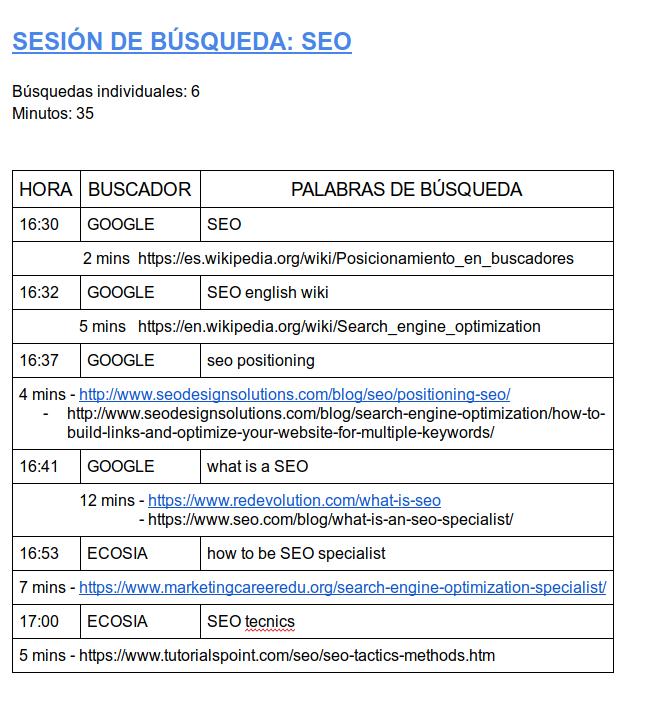
\includegraphics[width=1.2\textwidth]{seo-session.png}
	\end{subsection}
	\newpage
	
	\begin{section}{Detecci\'on de plagio}
		
		\begin{subsection}{Definici\'on.}
			Seg\'un \textit{plagiarism.org}\cite{plagiarism_org}, se considera plagio la acci\'on de presentar o usar trabajo de otro autor sin citarlo y sin especificar la fuente de procedencia.
			Seg\'un la RAE\cite{rae}, plagiar se define como la acci\'on de copiar obras ajenas y darlas a conocer como propias.\\
			
			En el \'area que nos compete, hablaremos de plagio en texto escrito, aunque tambien se considera plagio el uso de cualquier producci\'on de un autor sin su debida menci\'on. Cabe mencionar el caso de los archivos multimedia. Publicar im\'agenes, v\'ideos o fragmentos y composiciones de los mismos de otro autor sin su correspondiente fuente de procedencia tambi\'en es motivo de conflicto.
			
		\end{subsection}
		
		\begin{subsection}{Casos de plagio en la actualidad.}
			En 2015 se abri\'o una p\'agina de Facebook llamada \textit{Cabronazi} que empez\'o a publicar fotograf\'ias con mensajes graciosos. Tres a\~nos despu\'es cuenta con m\'as de 12 millones de seguidores y factura cerca de 370000 euros al a\~no. No obstante, detr\'as de este \'exito muchos usuarios se quejan de que la mayor\'ia de las publicaciones son plagio de otras en las redes sociales. Puede verse la discusi\'on en el peri\'odico \textit{El Confidencial}\cite{elconfidencial} .\\
			
			
			Un tema que genera m\'as controversia en la actualidad es el de Pedro S\'anchez, al que acusan de haber plagiado ciertas partes de su tesis doctoral. Tras haber publicado en internet dicha tesis, distintos medios han examinado el documento. Estos son los resultados seg\'un uno de esos medios\cite{sanchez}.
			
		\end{subsection}
		
		\begin{subsection}{M\'etodos para detectar plagio.}
			Existen numerosos m\'etodos para detectar plagio. Los m\'as frecuentes por su rapidez son los software de detecci\'on de plagio, aunque para usarlos se necesita los documentos en formato digital.\\ 
			\begin{itemize}
				
				
				\item \textbf{Cadenas de texto.} La mayor\'ia del software comercial se basa en la comparaci\'on de cadenas de texto. Usan una base de datos de documentos para enfrentar el documento sospechoso. Esto plantea un inconveniente, puede que la base de datos usada no sea suficientemente extensa o no contenga el documento plagiado. Se podr\'ia intentar a\~nadir la mayor cantidad de textos posibles para mejorar el contraste, pero esto supondr\'ia una penalizaci\'on en tiempo de c\'omputo.\\
				
				\item \textbf{Bolsas de palabras.} Una forma de reducir el tiempo ser\'ia usar comparaci\'on de bolsas de palabras. Una bolsa de palabras es un vector que representa las palabras de un texto. Por tanto, al usar bolsas de palabras estamos comprobando si dos textos usan el mismo vocabulario, obviando el orden en el que las palabras aparecen. Esto produce una reducci\'on de la eficacia del m\'etodo.
				
				Notar que sendos m\'etodos pueden ser mejorados con el uso de diccionarios de sin\'onimos y traductores para evitar la reformulaci\'on de oraciones y las traducciones.\\
				
				\item \textbf{Analizador de estilo.} Existen otras t\'ecnicas que proveen un an\'alisis m\'as profundo del texto, por ejemplo los analizadores de estilo. Este tipo de detectores analizan distintos aspectos en el discurso de un autor para hacer un perfil de escritura. Este perfil se puede caracterizar por la longitud de las oraciones, el uso de muletillas o de reformuladores del discurso. Cuando se introduce un nuevo documento en el sistema, se realizar un an\'alisis para encontrar estilos similares. Hay que notar que un analizador de estilo es sensible a idiomas, por tanto, las traducciones no literales de textos no ser\'ian detectadas por este m\'etodo.
				
			\end{itemize}
		\end{subsection}
		
		
		
		\begin{subsection}{Temporizaci\'on de b\'usqueda.}
			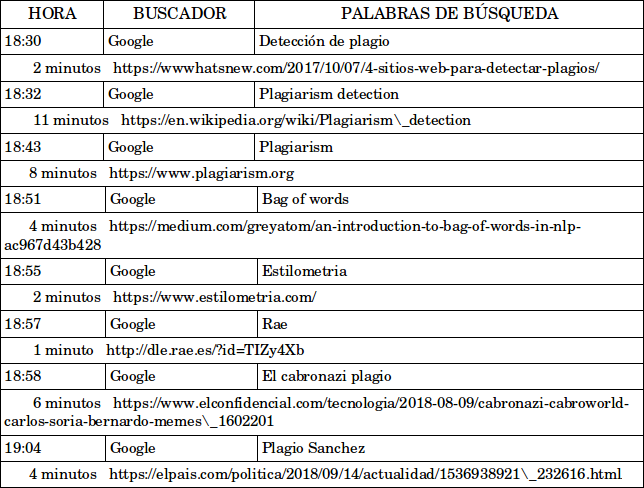
\includegraphics[width=1\textwidth]{plagio_tiempos.png}
		\end{subsection}
		
		
		
	\end{section}
	
	
	\newpage
	
	\bibliography{bibliografia.bib} %archivo citas.bib que contiene las entradas 
	\bibliographystyle{plain} % hay varias formas de citar
	
	
\end{document}














%%%%%%%%%%%%%%%%%%%%%%%%%%%%%%%%%%%%%%%%%
% Short Sectioned Assignment LaTeX Template Version 1.0 (5/5/12)
% This template has been downloaded from: http://www.LaTeXTemplates.com
% Original author:  Frits Wenneker (http://www.howtotex.com)
% License: CC BY-NC-SA 3.0 (http://creativecommons.org/licenses/by-nc-sa/3.0/)
%%%%%%%%%%%%%%%%%%%%%%%%%%%%%%%%%%%%%%%%%

%----------------------------------------------------------------------------------------
%	PACKAGES AND OTHER DOCUMENT CONFIGURATIONS
%----------------------------------------------------------------------------------------

\documentclass[paper=a4, fontsize=11pt]{scrartcl} % A4 paper and 11pt font size

% ---- Entrada y salida de texto -----

\usepackage[T1]{fontenc} % Use 8-bit encoding that has 256 glyphs
\usepackage[utf8]{inputenc}
%\usepackage{fourier} % Use the Adobe Utopia font for the document - comment this line to return to the LaTeX default

% ---- Idioma --------

\usepackage[spanish, es-tabla]{babel} % Selecciona el español para palabras introducidas automáticamente, p.ej. "septiembre" en la fecha y especifica que se use la palabra Tabla en vez de Cuadro

% ---- Otros paquetes ----

\usepackage{url} % ,href} %para incluir URLs e hipervínculos dentro del texto (aunque hay que instalar href)
\usepackage{amsmath,amsfonts,amsthm} % Math packages
%\usepackage{graphics,graphicx, floatrow} %para incluir imágenes y notas en las imágenes
\usepackage{graphics,graphicx, float} %para incluir imágenes y colocarlas

% Para hacer tablas comlejas
%\usepackage{multirow}
%\usepackage{threeparttable}

%\usepackage{sectsty} % Allows customizing section commands
%\allsectionsfont{\centering \normalfont\scshape} % Make all sections centered, the default font and small caps

\usepackage{fancyhdr} % Custom headers and footers
\pagestyle{fancyplain} % Makes all pages in the document conform to the custom headers and footers
\fancyhead{} % No page header - if you want one, create it in the same way as the footers below
\fancyfoot[L]{} % Empty left footer
\fancyfoot[C]{} % Empty center footer
\fancyfoot[R]{\thepage} % Page numbering for right footer
\renewcommand{\headrulewidth}{0pt} % Remove header underlines
\renewcommand{\footrulewidth}{0pt} % Remove footer underlines
\setlength{\headheight}{13.6pt} % Customize the height of the header

\numberwithin{equation}{section} % Number equations within sections (i.e. 1.1, 1.2, 2.1, 2.2 instead of 1, 2, 3, 4)
\numberwithin{figure}{section} % Number figures within sections (i.e. 1.1, 1.2, 2.1, 2.2 instead of 1, 2, 3, 4)
\numberwithin{table}{section} % Number tables within sections (i.e. 1.1, 1.2, 2.1, 2.2 instead of 1, 2, 3, 4)

\setlength\parindent{0pt} % Removes all indentation from paragraphs - comment this line for an assignment with lots of text

\newcommand{\horrule}[1]{\rule{\linewidth}{#1}} % Create horizontal rule command with 1 argument of height



\begin{document}
	
	\begin{titlepage}
		\centering
		
\includegraphics[width=0.8\textwidth]{decsai.jpeg}\par\vspace{1cm}
		{\scshape\LARGE Universidad de Granada \par}
		\vspace{1cm}
		{\scshape\Large Recuperaci\'on de Informaci\'on \par}
		\vspace{1.5cm}
		{\huge\bfseries Pr\'actica 1: B\'usqueda de informaci\'on en la web\par}
		\vspace{0.2cm}
		\noindent\rule{\textwidth}{2pt}
		\vspace{2cm}
		{\Large\itshape Miguel \'Angel Torres L\'opez y Luis Balderas Ruiz\par}
		
		\vfill
		
		% Bottom of the page
		{\large \today\par}
	\end{titlepage}
	
	\tableofcontents
	
	\newpage
	
	
	\begin{section}{Formatos de codificaci\'on}
		\begin{subsection}{Codificación de caracteres.}
			La codificación de caracteres es un método indispensable en la informática moderna, ya que nos permite comunicar y almacenar caracteres desde la representación binaria. No obstante, las técnicas de codificación de caracteres son algo más antigua, un ejemplo de ello es el código Morse. \\
			
			Desde el punto vista técnico, entendemos por una codificación de caracteres un sistema por el cual representamos caracteres identificándolos uno a uno con otros símbolos normados. 
		\end{subsection}
		
		\begin{subsection}{Formatos de codificación en informática.}
			En informática, uno de los primeros formatos de codificación que aparece es el ASCII. Este sistema de codificación usa un código de 7 bits, aunque los sistemas actuales están obligados a tomar 8 bits como unidad mínima de almacenamiento. Cada combinación representa un caracter, es decir, tiene 128 caracteres codificados. Este número era suficiente para representar textos en inglés y números, pero pronto quedó expuesta la necesidad de incluir otros caracteres, por ejemplo las caracteres latinos con tildes y otros signos de acentuación. \\
			
			Para ampliar la gama de caracteres y al mismo tiempo mantener la retrocompatibilidad UNICODE\cite{unicode}, el consorcio para la estandarización de codificación de caracteres, creo el formato UTF-8. Este formato es compatible con ASCII, pero difiere en el tamaño que ocupa un caracter. En UTF-8 los caracteres pueden ocupar 1, 2, 3 o 4 segmentos de 8 bits, siendo el primer segmento el mismo que el de ASCII.  Esta nueva codificiación permite representar hasta 1,112,064 caracteres, incluyendo alfabetos occidentales, orientales, símbolos matemáticos e incluso algunos de tipo privado.
			
			En cuanto a rapidez, el formato ASCII está por encima del UTF-8. Aunque a priori vemos que los caracteres tradicionales ocupan igual en los dos formatos, 1 segmento de 8 bits, hay ocasiones en que las posibilidades que nos da UTF-8 entorpezcan la lectura. Por ejemplo, supongamos que tenemos un string 'ABC'. En sendos formatos el string ocuparía 24 bits. Pero acceder al tercer elemento es más costoso en UTF-8, pues tenemos un tiempo adicional al tener que comprobar de que tamaño son los dos primeros caracteres.  \\
			
			Otra codificiación de UNICODE es el UTF-16. Este formato usa 1 o 2 segmentos de 16 bits por caracter, por tanto ya no es compatible con ASCII. No obstante, para lenguajes orientales, como el japonés, la mayoría de los caracteres pueden representarse con 16 bits, lo que aumenta la rapidez de lectura. \\ 
			
			Existe tambien el formato UTF-32, con la obligatoriedad de usar 1 segmento de 32 bits por caracter. Al igual que el anterior, no es compatible con ASCII y además es bastante más pesado e ineficiente, pues muchos bits son desaprovechados. Esto lo convierte en un formato poco usado en la actualidad. \\
			
			Por tanto, los dos formatos más comunes en la actualidad son UTF-8 y ASCII, aunque poco a poco se está incorporando el formato UTF-16 por compatibilidad con los ordenadores de origen asiático.
			
			
		\end{subsection}
		
		\begin{subsection}{Sistemas operativos y sus formatos}
			En esta sección haremos un repaso de los principales sistemas operativos y los formatos de codificiación bajo los que trabajan:
			
			\begin{itemize}
				\item \textbf{Windows}. Fue uno de los primeros sistemas en actualizar el formato de codificación. Actualmente utiliza UTF-16, pero sigue sin funcionar de forma óptima con UTF-8.
				
				\item \textbf{Linux}. Funciona en su mayor parte con UTF-8, aunque dispone de herramientas para cambiar el formato de un archivo. Una de ellas es el comando de termina iconv, que convierte una entrada con un formato a una salida con otro distinto.   
				
				\item \textbf{Mac}. Al igual que Linux trabaja con UTF-8.
				
			\end{itemize}
		\end{subsection}
		
		\begin{subsection}{Temporizaci\'on de b\'usqueda.}
			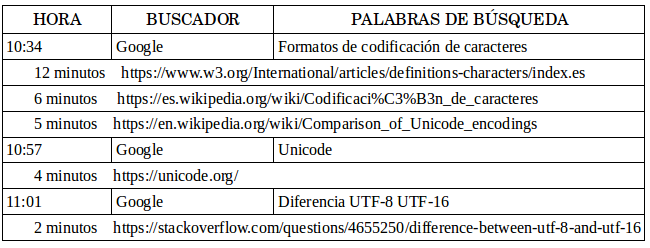
\includegraphics[width=1\textwidth]{codificacion_tiempos.png}
		\end{subsection}
		
	\end{section}
	
	\newpage
	
	\begin{section}{SEO.}
		SEO (Search Engine Optimization) o posicionamiento en buscadores es uno de los conceptos claves de la industria digital. Tanto el posicionamiento en sí como la profesión que subyace, el SEO se ha convertido en algo que todo empresario, experto en marketing o incluso \textit{influencer} desea entender, manejar o, en el peor de los casos, contratar. En este pequeño informe tratamos de clarificar qué es exactamente el posicionamiento en buscadores desde un punto de vista técnico y por qué es necesario para los afamados \textit{e-business}, así como cuál es el camino para convertirse en un profesional SEO.
		
		\subsection{SEO como herramienta de marketing digital}
		Tal y como \cite{redevolution} menciona, SEO es ``el nombre que se le da a la actividad que intenta mejorar los rankings en las búsquedas", es decir, la posición en la que una página web aparece tras realizar una búsqueda con palabras clave (keywords) relacionadas con dicha web. Hay que añadir que, pese a que nuestra web tenga un gran posicionamiento en buscadores, fruto de un trabajo constante que más abajo desarrollamos, los anuncios (que reportan beneficios a Google u otros buscadores) aparecerán siempre antes. Por tanto, el objetivo del SEO es mejorar la posición de una página dentro de las denominadas \textit{búsquedas orgánicas} o \textit{naturales}. Las empresas tienen especial interés en estar presentes de forma conveniente en buscadores y redes dado que recibirán más visitas y, eventualmente, esas visitas se convierten en ventas o beneficios. Por tanto, a pesar de su peso técnico-informático, SEO es una estrategia de marketing en Internet. Como se puede leer en \cite{wiki}, como estrategia de marketing digital, "SEO considera cómo funcionan los buscadores, es decir, los algoritmos de búsqueda subyacentes que dictan el comportamiento de la búsqueda". Gran papel juegan las palabras clave o \textit{keywords} y los enlaces. Además, en los últimos tiempos se están desarrollando nuevos productos entorno al SEO móvil dado que las búsquedas móviles han superado a las mismas realizadas en PCs. \\
		
		El auge del posicionamiento en buscadores tiene una gran relación con Google. Desde que Larry Page y Sergey Brin idearon \textit{Backrub} y su algoritmo \textit{PageRank}, basado en la cantidad e importancia de los llamados \textit{backlinks o inbound links} (enlaces que recibe una web desde otra o, en otras palabras, la cantidad de páginas que enlazan con el sitio web a través de un vínculo \cite{backl}), los distintos propietarios de páginas se percataron de la importancia del posicionamiento y trataron de 'inflar' su PageRank. Ante los intentos de manipular fraudulentamente el PageRank por medio de SPAM, Google desarrolló en 2012 un algoritmo llamado \textit{Google Penguin}, que evalúa la calidad de los links de los que proceden las páginas web.
		
		\subsection{Herramientas SEO}
		
		Como dice \cite{seoc}, existen multitud de herramientas que nos ayudan a conocer el posicionamiento en buscadores de una página o negocio online. Entre ellas destacan:
		\begin{itemize}
			\item Google Analytics: Genera estadística con multitud de información interesante para nuestro negocio,  como cuándo y cuántos usuarios navegan por nuestra web.
			\item Webmaster Tools
			\item Bing Webmaster Tools
			\item Sitemap XMl Generator
			\item Herramienta de palabras clave Adwords: Nos ayuda a crear contenido que nos permitan generar textos de calidad y originales.
			\item Google Trends: Nos ayuda a buscar tendencias entre los usuarios en torno a un producto o servicio
		\end{itemize}
		
	\end{section}
	
	\newpage
	
	\begin{section}{Detecci\'on de plagio}
		
		\begin{subsection}{Definici\'on.}
			Seg\'un \textit{plagiarism.org}\cite{plagiarism_org}, se considera plagio la acci\'on de presentar o usar trabajo de otro autor sin citarlo y sin especificar la fuente de procedencia.
			Seg\'un la RAE\cite{rae}, plagiar se define como la acci\'on de copiar obras ajenas y darlas a conocer como propias.\\
			
			En el \'area que nos compete, hablaremos de plagio en texto escrito, aunque tambien se considera plagio el uso de cualquier producci\'on de un autor sin su debida menci\'on. Cabe mencionar el caso de los archivos multimedia. Publicar im\'agenes, v\'ideos o fragmentos y composiciones de los mismos de otro autor sin su correspondiente fuente de procedencia tambi\'en es motivo de conflicto.
			
		\end{subsection}
		
		\begin{subsection}{Casos de plagio en la actualidad.}
			En 2015 se abri\'o una p\'agina de Facebook llamada \textit{Cabronazi} que empez\'o a publicar fotograf\'ias con mensajes graciosos. Tres a\~nos despu\'es cuenta con m\'as de 12 millones de seguidores y factura cerca de 370000 euros al a\~no. No obstante, detr\'as de este \'exito muchos usuarios se quejan de que la mayor\'ia de las publicaciones son plagio de otras en las redes sociales. Puede verse la discusi\'on en el peri\'odico \textit{El Confidencial}\cite{elconfidencial} .\\
			
			
			Un tema que genera m\'as controversia en la actualidad es el de Pedro S\'anchez, al que acusan de haber plagiado ciertas partes de su tesis doctoral. Tras haber publicado en internet dicha tesis, distintos medios han examinado el documento. Estos son los resultados seg\'un uno de esos medios\cite{sanchez}.
			
		\end{subsection}
		
		\begin{subsection}{M\'etodos para detectar plagio.}
			Existen numerosos m\'etodos para detectar plagio. Los m\'as frecuentes por su rapidez son los software de detecci\'on de plagio, aunque para usarlos se necesita los documentos en formato digital.\\ 
			\begin{itemize}
				
				
				\item \textbf{Cadenas de texto.} La mayor\'ia del software comercial se basa en la comparaci\'on de cadenas de texto. Usan una base de datos de documentos para enfrentar el documento sospechoso. Esto plantea un inconveniente, puede que la base de datos usada no sea suficientemente extensa o no contenga el documento plagiado. Se podr\'ia intentar a\~nadir la mayor cantidad de textos posibles para mejorar el contraste, pero esto supondr\'ia una penalizaci\'on en tiempo de c\'omputo.\\
				
				\item \textbf{Bolsas de palabras.} Una forma de reducir el tiempo ser\'ia usar comparaci\'on de bolsas de palabras. Una bolsa de palabras es un vector que representa las palabras de un texto. Por tanto, al usar bolsas de palabras estamos comprobando si dos textos usan el mismo vocabulario, obviando el orden en el que las palabras aparecen. Esto produce una reducci\'on de la eficacia del m\'etodo.
				
				Notar que sendos m\'etodos pueden ser mejorados con el uso de diccionarios de sin\'onimos y traductores para evitar la reformulaci\'on de oraciones y las traducciones.\\
				
				\item \textbf{Analizador de estilo.} Existen otras t\'ecnicas que proveen un an\'alisis m\'as profundo del texto, por ejemplo los analizadores de estilo. Este tipo de detectores analizan distintos aspectos en el discurso de un autor para hacer un perfil de escritura. Este perfil se puede caracterizar por la longitud de las oraciones, el uso de muletillas o de reformuladores del discurso. Cuando se introduce un nuevo documento en el sistema, se realizar un an\'alisis para encontrar estilos similares. Hay que notar que un analizador de estilo es sensible a idiomas, por tanto, las traducciones no literales de textos no ser\'ian detectadas por este m\'etodo.
				
			\end{itemize}
		\end{subsection}
		
		
		
		\begin{subsection}{Temporizaci\'on de b\'usqueda.}
			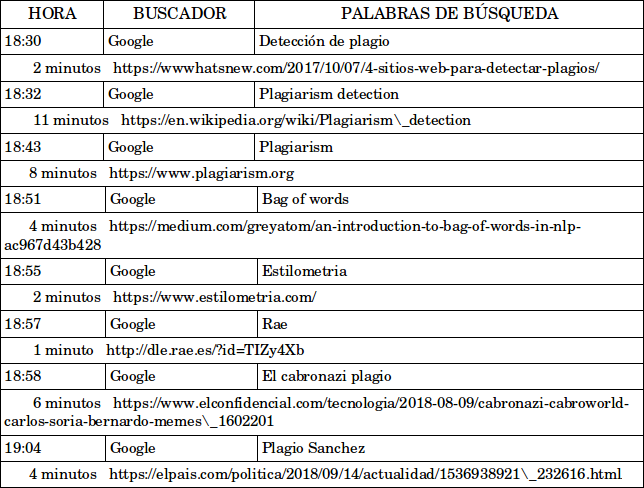
\includegraphics[width=1\textwidth]{plagio_tiempos.png}
		\end{subsection}
		
		
		
	\end{section}
	
	
	\newpage
	
	\bibliography{bibliografia.bib} %archivo citas.bib que contiene las entradas 
	\bibliographystyle{plain} % hay varias formas de citar
	
	
\end{document}